
\section{Úvod}
\subsection{View Model Data Binding}
\begin{frame}[dart-main]{View Model NO Data Binding}
	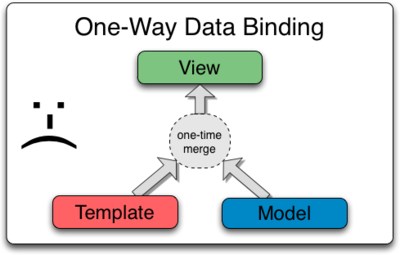
\includegraphics[scale=0.7]{images/no-data-binding.png}
\end{frame}
\begin{frame}[dart-main]{View Model Data Binding}
	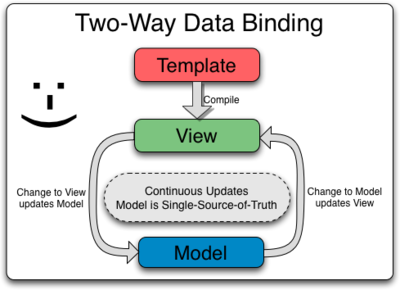
\includegraphics[scale=0.7]{images/data-binding.png}
\end{frame}

\section{Dart}
\subsection{Základ}
\begin{frame}[dart-main]{Základ}
	\begin{columns}[T]
		\begin{column}{.5\textwidth}
			\begin{itemize}
				\item product by Google
				\item objektovo orientovaný jazyk
				\item prvky Java-y, JavaScript-u aj Scala-y
				\item Closures
				\item \url{https://www.dartlang.org/}
			\end{itemize}
		\end{column}
		\begin{column}{.5\textwidth}
			% \begin{block}{Your image}
			% Your image included here
			
\includegraphics[scale=0.3]{images/dart-logo.png}\\
			
\includegraphics[scale=0.05]{images/google.png}
			% \end{block}
		\end{column}
	\end{columns}
\end{frame}

\subsection{Ukážka zdrojového kódu}
\begin{frame}[fragile]
	\begin{verbatim}
import 'dart:html';

InputElement toDoInput;
UListElement toDoList;

void main() {
  toDoInput = query('#to-do-input');
  toDoList = query('#to-do-list');
  toDoInput.onChange.listen(addToDoItem);
}

void addToDoItem(Event e) {
  var newToDo = new LIElement();
  newToDo.text = toDoInput.value;
  toDoInput.value = '';
  toDoList.children.add(newToDo);
}
	\end{verbatim}
\end{frame}

\begin{frame}[fragile]
	\begin{verbatim}
class Point {
  num x;
  num y;

  Point(this.x, this.y);

  // Named constructor
  Point.fromJson(Map json) {
    x = json['x'];
    y = json['y'];
  }
  num vectorSize() => sqrt(pow(x, 2) + pow(y, 2));  
}

void main(){
  Map<String, num> json = {"x" : 23, "y" : 47};
  var point = new Point.fromJson(json);
}
	\end{verbatim}
\end{frame}

\section{React}
\subsection{Zhruba o React-e}
\begin{frame}[react-main]{Zhruba o React-e}
	\begin{columns}[T]
		\begin{column}{.5\textwidth}
			\begin{itemize}
				\item Produkt Facebook-u a Istagram-u
				\item Komponentová architektúra
				\item Odľahčený DOM
					\begin{itemize}
						\item Manipulácia s DOM-om je drahá
						\item Vlastná štrukúra udržuje internú verziu DOM-u
						\item Iba konštanté zrýchlenie - avšak vysoká konštanta
					\end{itemize}
			\end{itemize}
		\end{column}
		\begin{column}{.5\textwidth}
			% \begin{block}{Your image}
			% Your image included here
			
\includegraphics[scale=0.3]{images/react-logo.png}\\
			
\includegraphics[scale=0.2]{images/facebook.png}\\
			
\includegraphics[scale=0.15]{images/istagram.png}
			% \end{block}
		\end{column}
	\end{columns}
\end{frame}

\subsection{Základná idea}
\begin{frame}[react-idea]{Základná idea}
	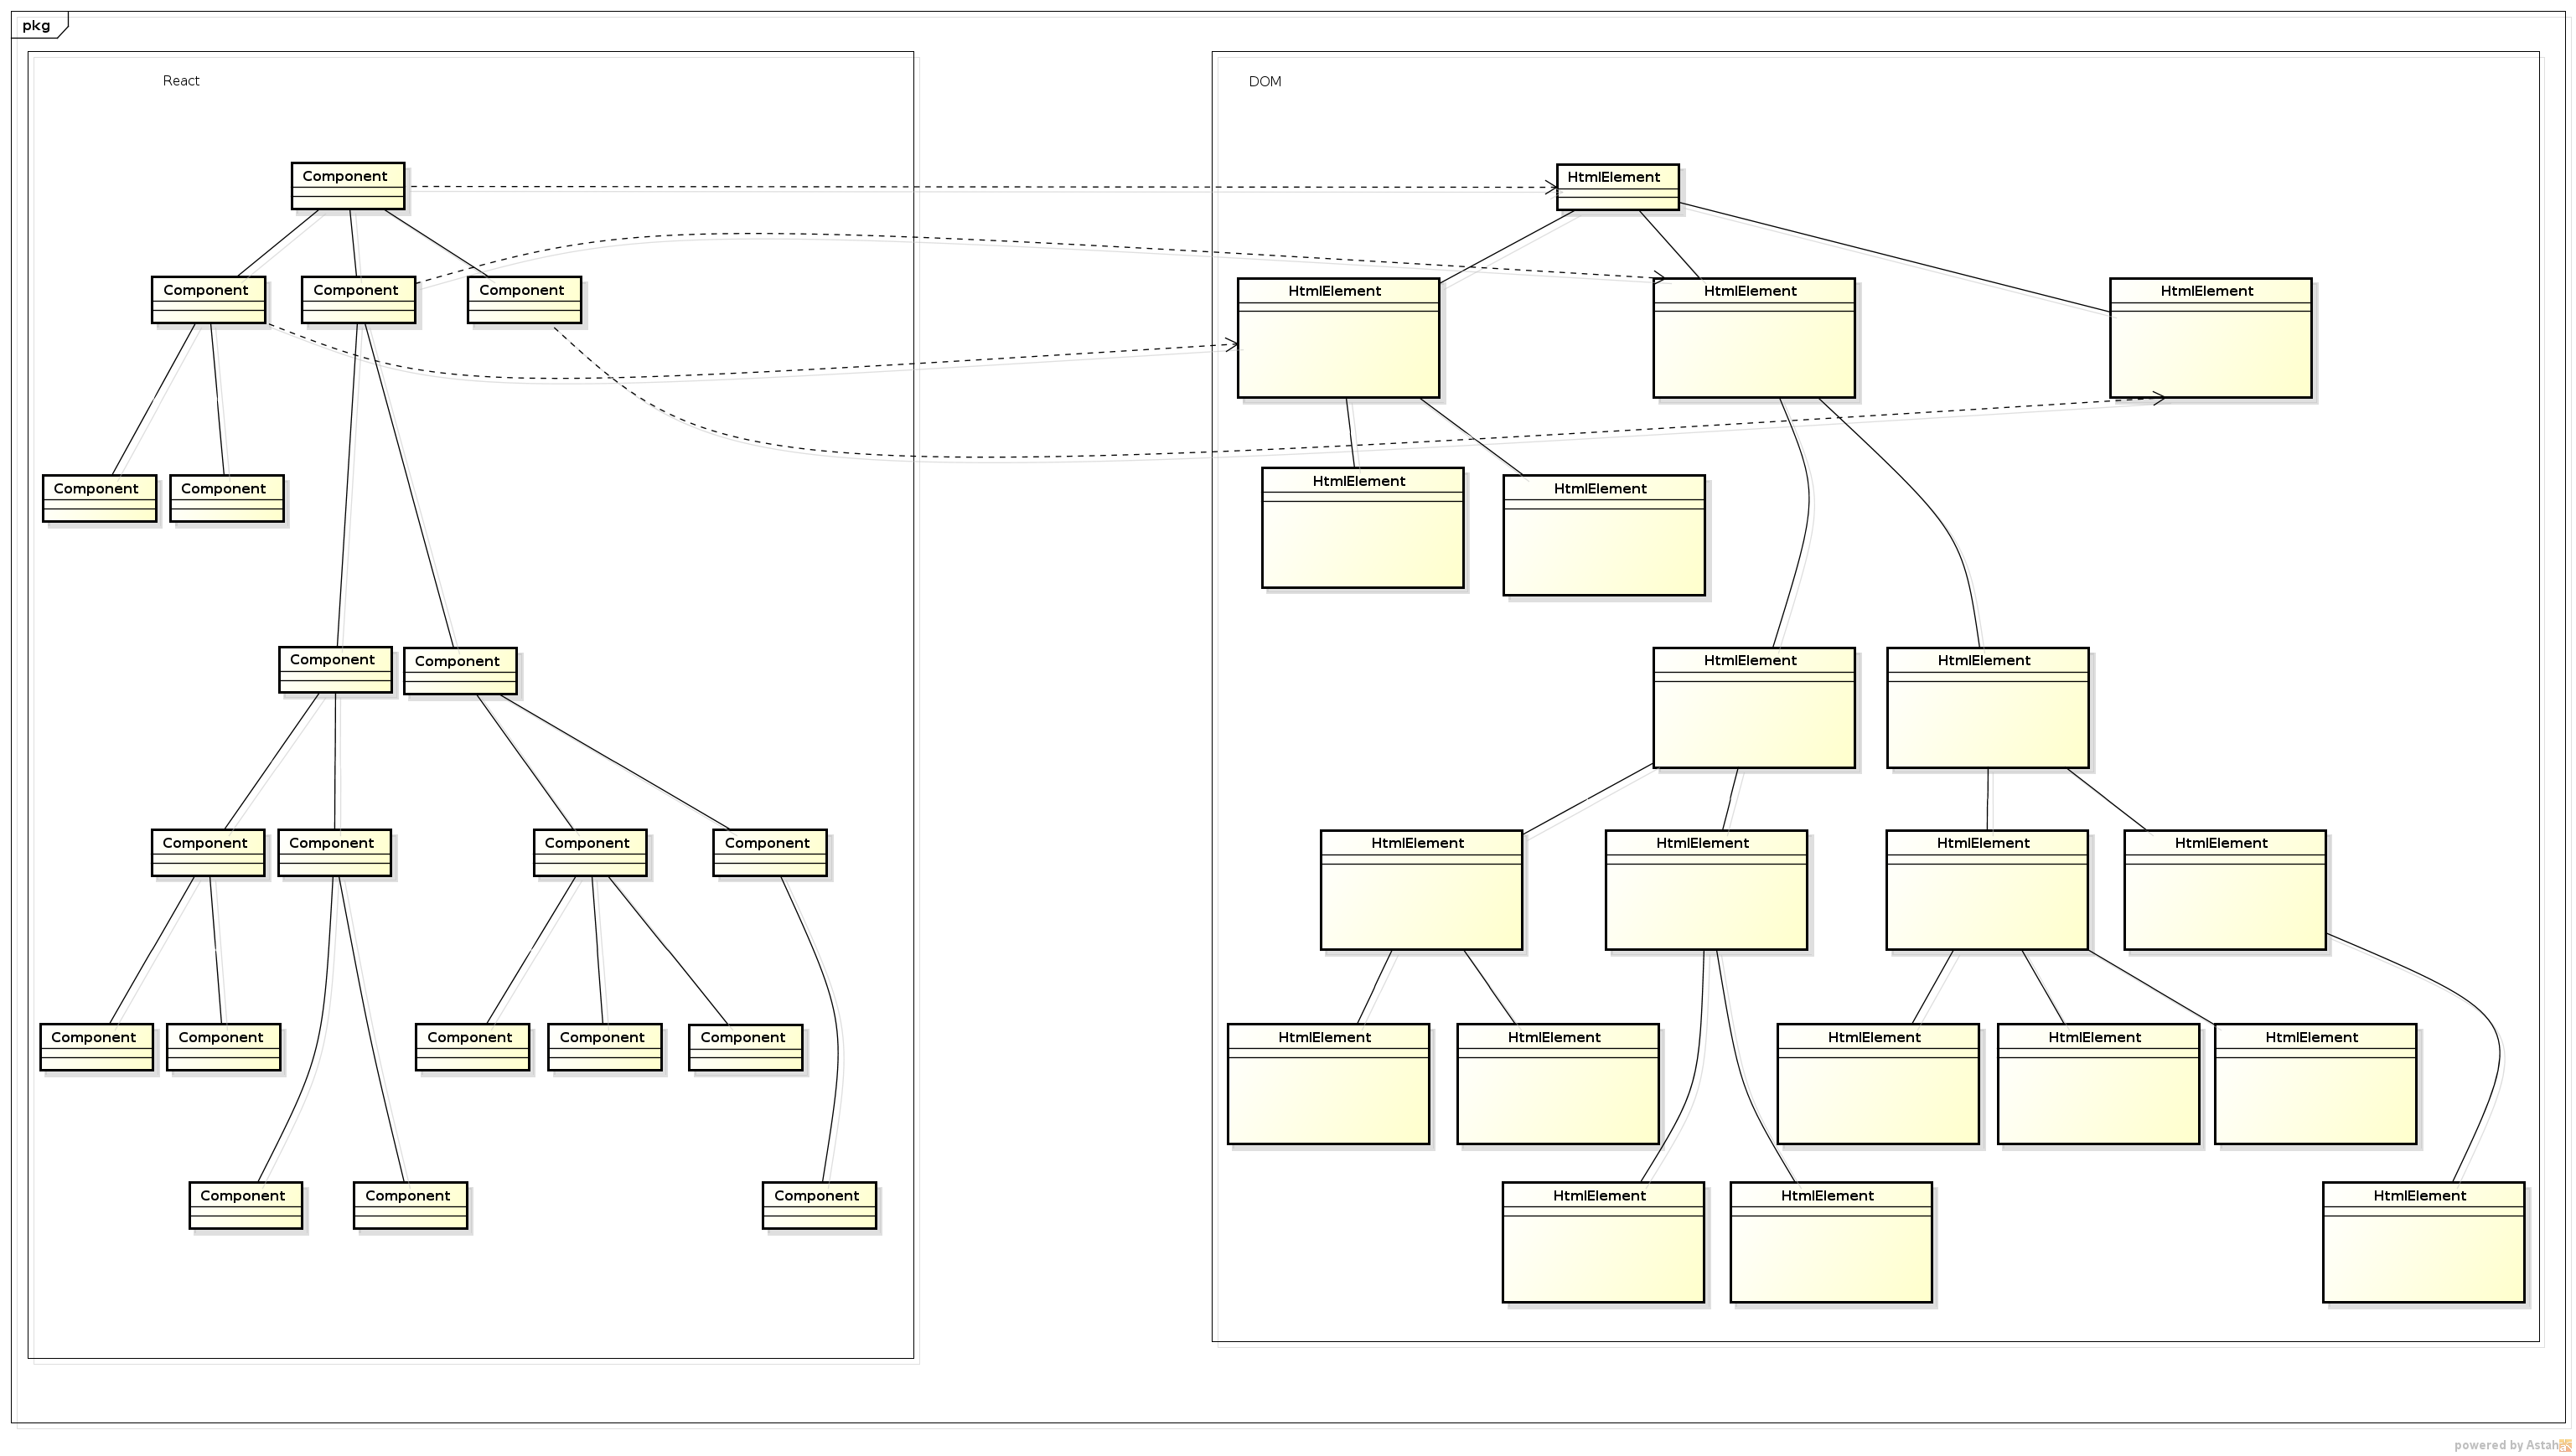
\includegraphics[width=\linewidth,height=\textheight,keepaspectratio]{images/react-dom.png}
\end{frame}

\begin{frame}[react-aditions]{Drobné vylepšenia}
	\begin{itemize}
		\item Browser compatibility
		\item Synthetic events
		\item Mixins
	\end{itemize}
\end{frame}

\section{AngularJS}
\subsection{Zhruba o AngularJS}
\begin{frame}[angular-main]{Zhruba o AngularJS}
	\begin{columns}[T]
		\begin{column}{.5\textwidth}
			\begin{itemize}
				\item product by Google
				\item skôr template-ovací jazyk
				\item \url{http://angularjs.org/}
			\end{itemize}
		\end{column}
		\begin{column}{.5\textwidth}
			% \begin{block}{Your image}
			% Your image included here
			
\includegraphics[scale=0.3]{images/angular-logo.png}\\
			
\includegraphics[scale=0.05]{images/google.png}
			% \end{block}
		\end{column}
	\end{columns}
\end{frame}

